\thispagestyle{empty}

\rule{\textwidth}{0pt}

\vfill

\ifdraft{%
  El documento
  \href{https://www.tec.ac.cr/sites/default/files/media/doc/requisitos_trabajos_finales_graduacion_2021.pdf}%
  {Requisitos para la entrega de Trabajos Finales de Graduación} a las
  bibliotecas del TEC indica que usted debe incluir la licencia de
  Creative Commons en la página siguiente de la portada.

  Asegúrse entonces de \href{https://creativecommons.org/choose/?lang=es}%
  {elegir la licencia correcta}, y ajustar el texto abajo a su selección.

  Es necesario que
  \href{https://creativecommons.org/about/downloads/}{descargue el
    ícono} correcto en formato vectorial, y lo coloque en el
  directorio \code{fig/}.%
}



\vfill


\framebox[\textwidth]{
  \footnotesize
  \parbox{0.98\textwidth}{%
    \begin{center} %
      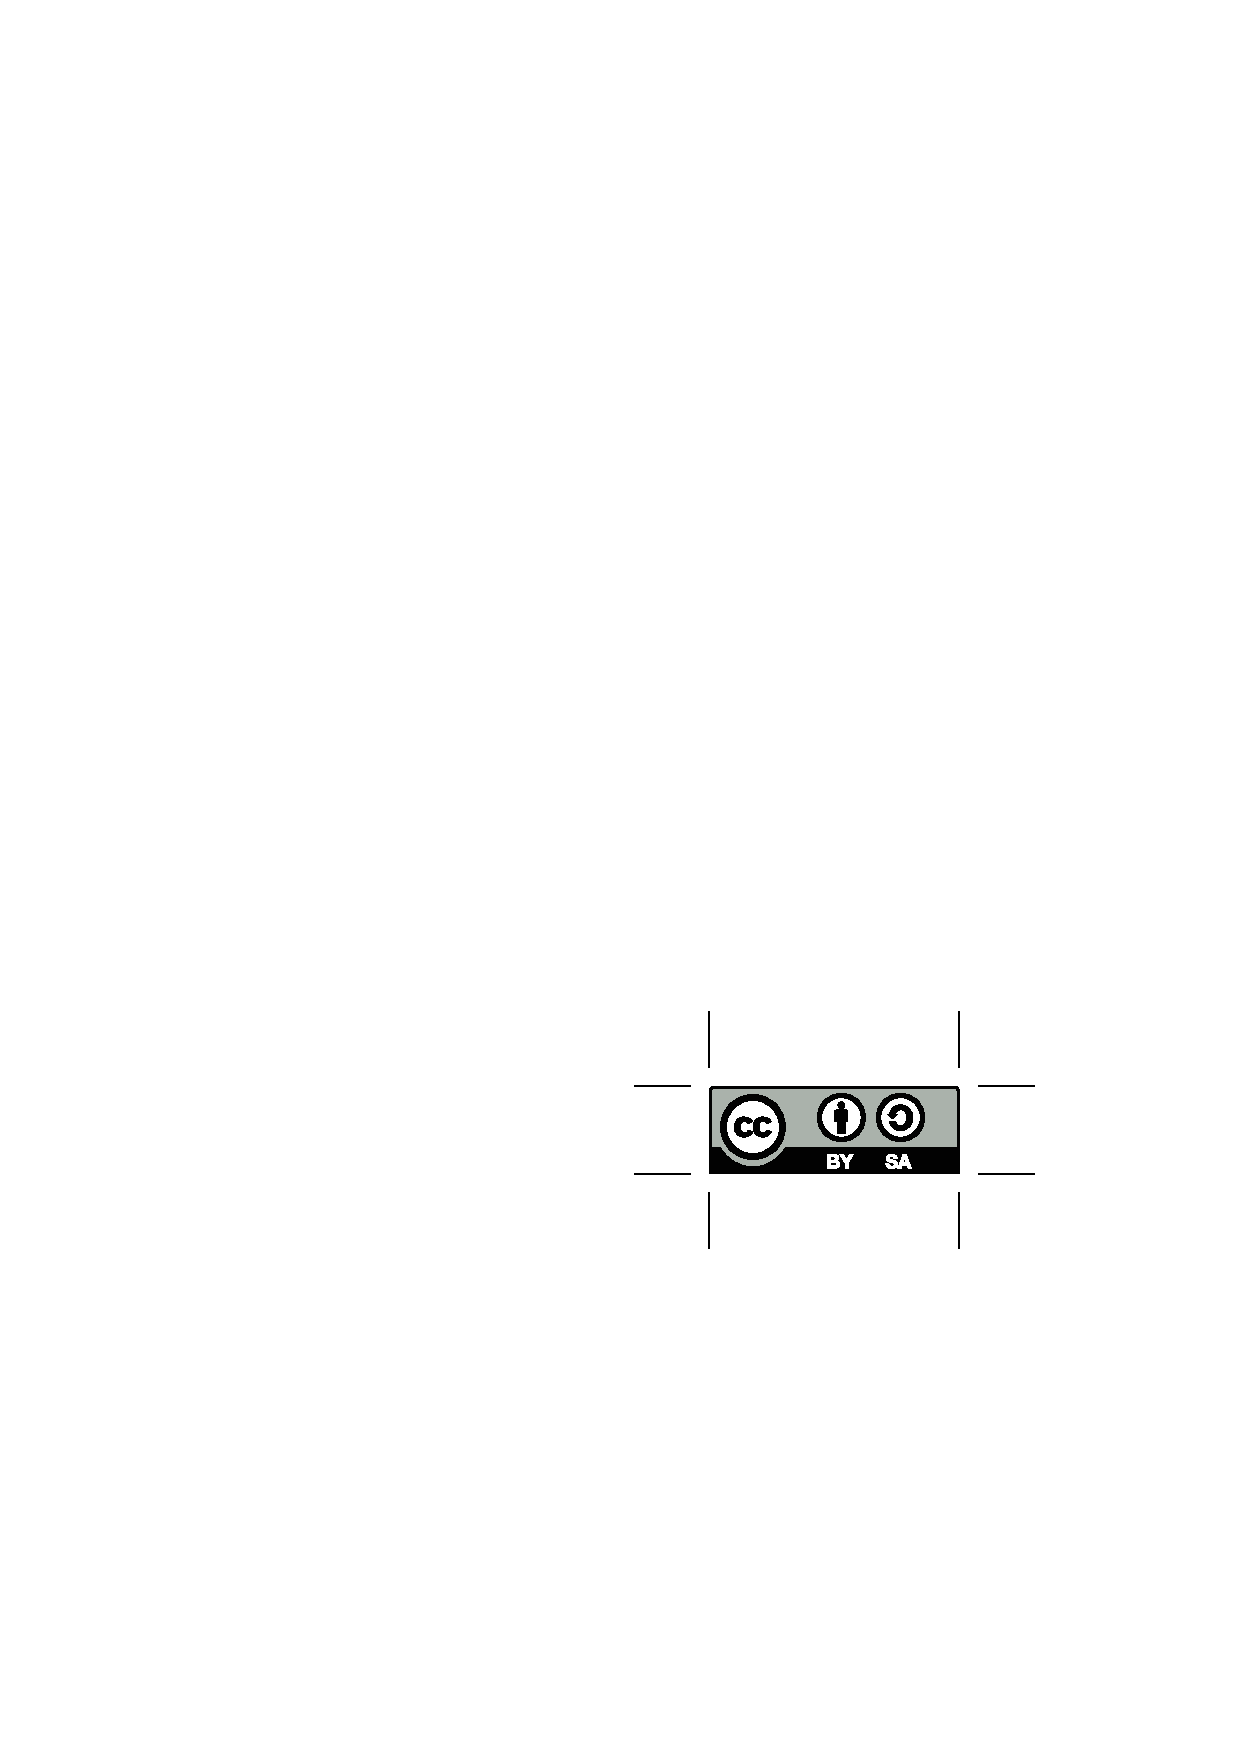
\includegraphics[scale=1]{by-sa} %
    \end{center} %
    
    Este trabajo titulado \emph{\thesisFlatTitle{}} por \thesisAuthor{}, se
    encuentra bajo la Licencia Creative Commons
    \href{http://creativecommons.org/licenses/by-sa/4.0/?ref=chooser-v1}%
    {Atribución-ShareAlike 4.0 International}.
    
    Para ver una copia de esta Licencia, visite
    \url{http://creativecommons.org/licenses/by-sa/4.0/}.\bigskip
    
    \copyright \the\year \hfill%
    \thesisAuthor \hfill%
    \thesisInstitution
  }
}
